%!TEX root = ../doc.tex
\chapter{Ist Analyse}
\label{sec:istanalyse}
\section{ImagineCargo}
ImagineCargo operiert im DACH-Raum (Deutschland, Österreich und Schweiz) und bietet die nachhaltige Expresskurier-Dienstleistung in 15 Städten an. Das Startup wurde im Oktober 2014 von Nick Blake gegründet und beschäftigt zur Zeit acht bis neun Mitarbeiter. Für das Unternehmen wurde ein Business Model Canvas erstellt, welches in der Abbildung \ref{fig1:businessmodelcanvas} zu sehen ist. Business Model Canvas sind Vorlagen, um neue Prozesse zu entwickeln bzw. bestehende Prozesse zu dokumentieren.
\begin{figure}[ht]
	\centering
  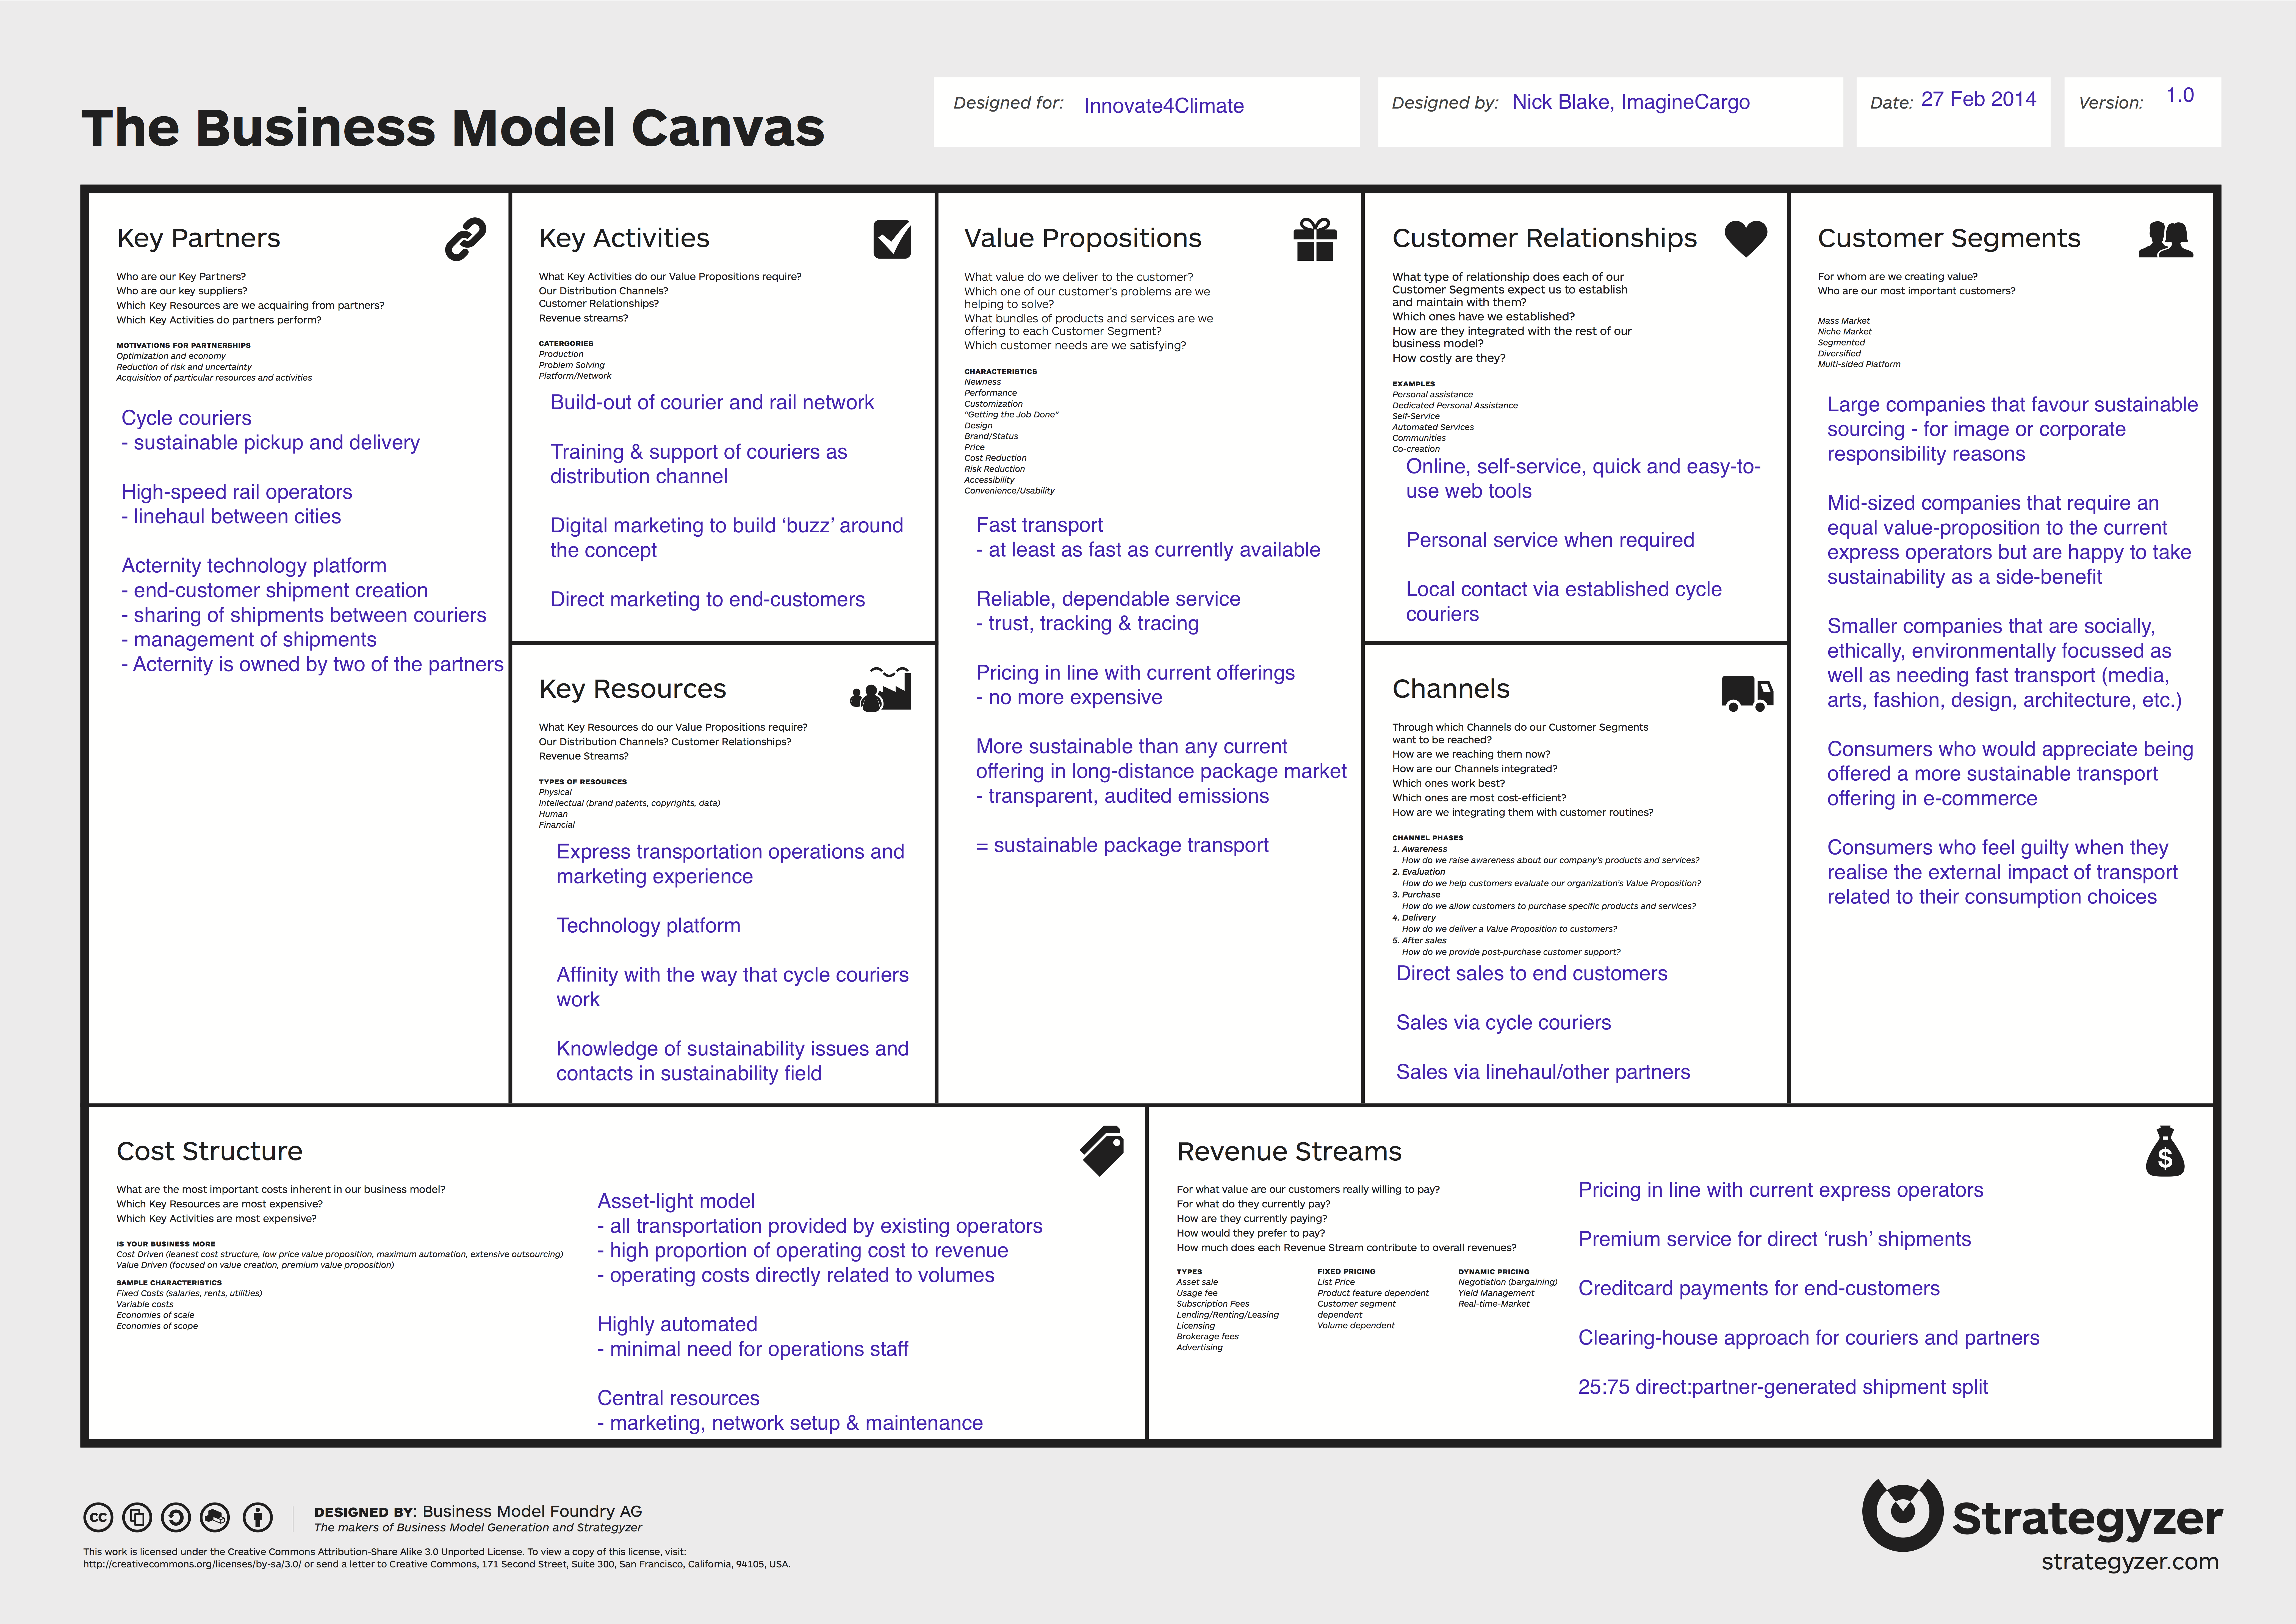
\includegraphics[width=0.88\textwidth]{images/businessModelCanvas.png}
	\caption{Business Model Canvas von Imagine Cargo}
	\label{fig1:businessmodelcanvas}
\end{figure}
 Die Mitarbeiter von ImagineCargo haben rotierend die Rolle des Disponenten, welcher Aufträge per Mail oder Telefon annimmt und alle notwendigen Schritte für eine erfolgreiche Lieferung ausführt. Auf der Webseite von Imagine Cargo exisitiert eine \textit{wufoo-Form} mit welchem über HTML 5 Form Elemente die benötigten Informationen eingegeben werden können und danach per Mail an den zuständigen Disponenten geschickt werden. Der Prozess wird im Kapitel \ref{subsec:prozess} genauer beschrieben.


\subsection{Prozesse}
\label{subsec:prozess}
LoBo wurde ursprünglich für die Verwaltung und Koordinierung von Fahrradkurieren in \textbf{einer} Stadt entwickelt. In LoBo wird mit einem Polygon auf einer Karte das Versorgungsgebiet markiert. Damit wird überprüft ob eine Start- beziehungsweise Zieladresse zugelassen ist. Obwohl in einer LoBo-Instanz mehrere Polygone respektive mehrere Versorgungsgebiete konfiguriert werden können, bietet LoBo nicht sonderlich viele Funktionen an, um eine Dienstleistung zwischen diesen Gebieten zu ermöglichen. Das grundsätzliche Problem besteht in der Berechnung der Dauer des Auftrages. Für das bessere Verständnis sei hier ein Beispiel beschrieben. Eine Zugfahrt von Zürich HB nach Berlin Hbf dauert ca. acht Stunden und elf Minuten. Ein Auftrag für ein Paket aus dem Zürcher Kreis 4 nach Wedding in Berlin dauert inkl. Bahntransport ca. zehn Stunden. Wenn besagter Auftrag um acht Uhr morgens gestartet wird, trifft das Paket um ca. 18 Uhr an seinem Bestimmungsort ein. Die Öffnungszeiten des Berliner Kuriers sind von montags bis freitags von 07:30 Uhr bis 20:00 Uhr und dementsprechend kein Hindernis für das Paket nach Berlin Wedding. Wenn der gleiche Auftrag um 13:00 Uhr gestartet werden soll, wird das Paket in Berlin aber nicht mehr vom Hauptbahnhof abgeholt. Um diese Berechnungen möglich zu machen, wurden in LoBo sogenannte Kreuztabellen implementiert. In diesen Kreuztabellen werden die Reisezeiten zwischen den verschiedenen Versorgungsgebieten eingetragen, wodurch die Berechnung der Gesamtdauer eines Auftrages möglich wird. Zusätzlich zu den Kreuztabellen sind einige weitere Schritte notwendig, um einen Auftrag korrekt im System einzutragen. In der Abbildung \ref{fig1:currentprocess} ist der Prozess schematisch dargestellt.

\begin{figure}[ht]
	\centering
  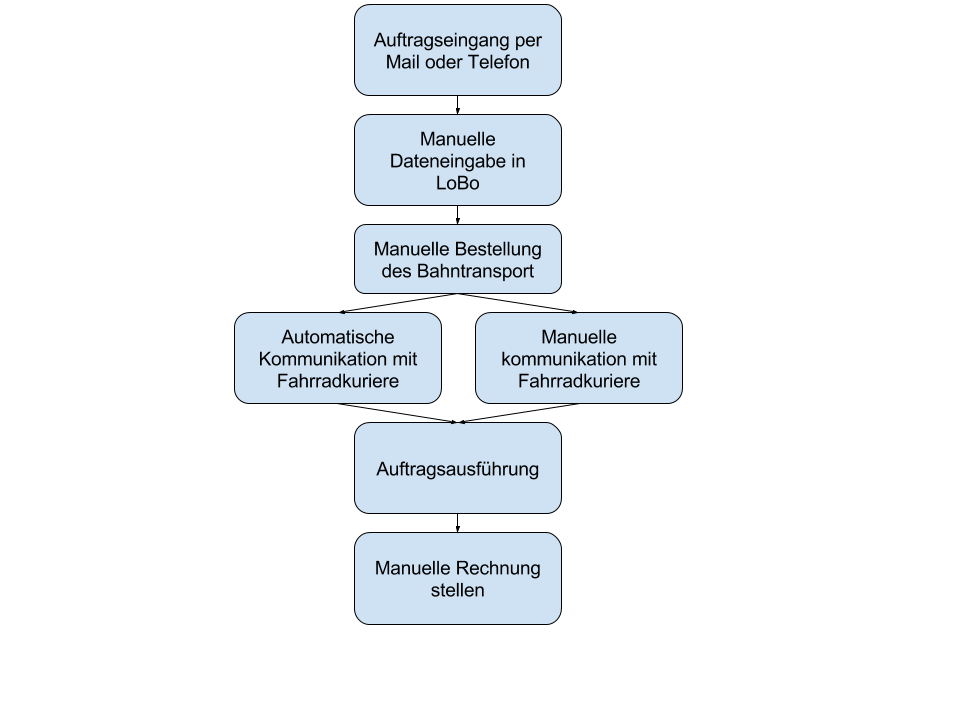
\includegraphics[width=0.88\textwidth]{images/currentProcess.png}
	\caption{Aktueller Prozess für die Erstellung eines Auftrages}
	\label{fig1:currentprocess}
\end{figure}

Bei der manuellen Dateneingabe in LoBo muss der korrekte Bahnhof der Stadt, in der eine Lieferung startet und in der sie ankommen soll, als zusätzliche Stopps eingetragen werden. Dadurch weiss der zuständige Fahrradkurier, wohin das Paket soll. Für die Start- und Zielstadt sind in den meisten Fällen unterschiedliche Fahrradkurierunternehmen zuständig. Deshalb muss dem Auftrag, sobald der Fahrradkurier der Startstadt das Paket an den Bahnhof gebracht hat, der zuständige Fahrradkurier der Zielstadt zugewiesen werden. Dieser Umstand wird in Kauf genommen, damit am Ende des Auftrages die Abrechnung immer noch korrekt funktioniert. Bevor der Auftrag überhaupt startet, muss für das Paket ein Ticket bei der zuständigen Bahngesellschaft bestellt werden. In Deutschland wird der Verkauf von diesen Tickets von time:matters\footnote{time:matters ist eine Tochtergesellschaft von Lufthansa Cargo, welche das Monopol auf das Transportieren von Pakete in Deutschland besitzt \url{http://www.time-matters.com/}} angeboten, aber nicht über eine API. Dies wird vom zuständigen Disponenten manuell ausgeführt und dann den beauftragten Fahrradkurieren übermittelt.


\section{Marktanalyse}
Beim Versuch einen Überblick über die vorhandenen Softwarelösungen auf dem Markt zu bekommen, sind viele Softwarelösungen für Speditionen in den Suchresultaten aufgetaucht. Viele dieser Softwarelösungen sind nur schon unbrauchbar, weil sie auf einer klassischen Client-Server-Architektur mit ausführbaren Programmen aufbauen. Die wenigen Angebote, welche eine webbasierte Benutzeroberfläche anbieten, sind aber durch den starken Fokus auf Spedition unbrauchbar. Diese Tools sind bessem geeignet, eine möglichst effiziente Traveling-Salesman-Route zu berechnen, als für Kunden, welche zum ersten mal versuche, ein Paket mit einem Expresskurier zu verschicken. Die zwei vielversprechendsten Lösungen werden im Folgenden kurz vorgestellt.

\subsection{Deliveo}
Deliveo ist eine Software für Kurierdienste und KEP-Dienstleister mit dem Fokus auf motorisierte Fahrzeuge und Fahrräder. Die Benutzeroberfläche von Deliveo macht einen vielversprechenden Eindruck\footnote{ Siehe Abbildung \ref{fig1:deliveomask}} und bietet eine grosse Anzahl an Funktionen. Im Folgende eine nicht abgeschlossene Liste mit Funktionen von Deliveo\footnote{ Informationen direkt von der Webseite des Herstellers. \url{http://deliveo.eu/}}.
\begin{itemize}
	\item Das ganze System ist mehrsprachig.
	\item Abrechnung mit dem Kurier (Nachnahme-Preise, Servicepreise und zurückgeholte Dokumente).
	\item Positionsanzeige des Kuriers
	\item Gut entwickeltes API System für die Kommunikation mit anderen Systemen, oder zur Unterstützung der unabhängigen Entwicklungen des Kurierdienstes.
	\item Paket-Betrieb (Aufnahme und Auslieferung) mittels Barcode-Leser mit Smartphone-Kamera
\end{itemize}
Die Benutzeroberfläche welche die Erstellung eines neuen Auftrags ermöglicht, scheint den Bedürfnissen welche in Kapitel \ref{sec:personastories} beschrieben sind, zu einem grossen Teil gerecht zu werden\footnote{ Siehe Abbildung \ref{fig1:deliveonew}}. Die Handhabung macht einen einfachen Eindruck und aus Sicht des Benutzer wirkt es angenehmer, als die Eingabemaske von LoBo.

\begin{figure}[ht]
	\centering
  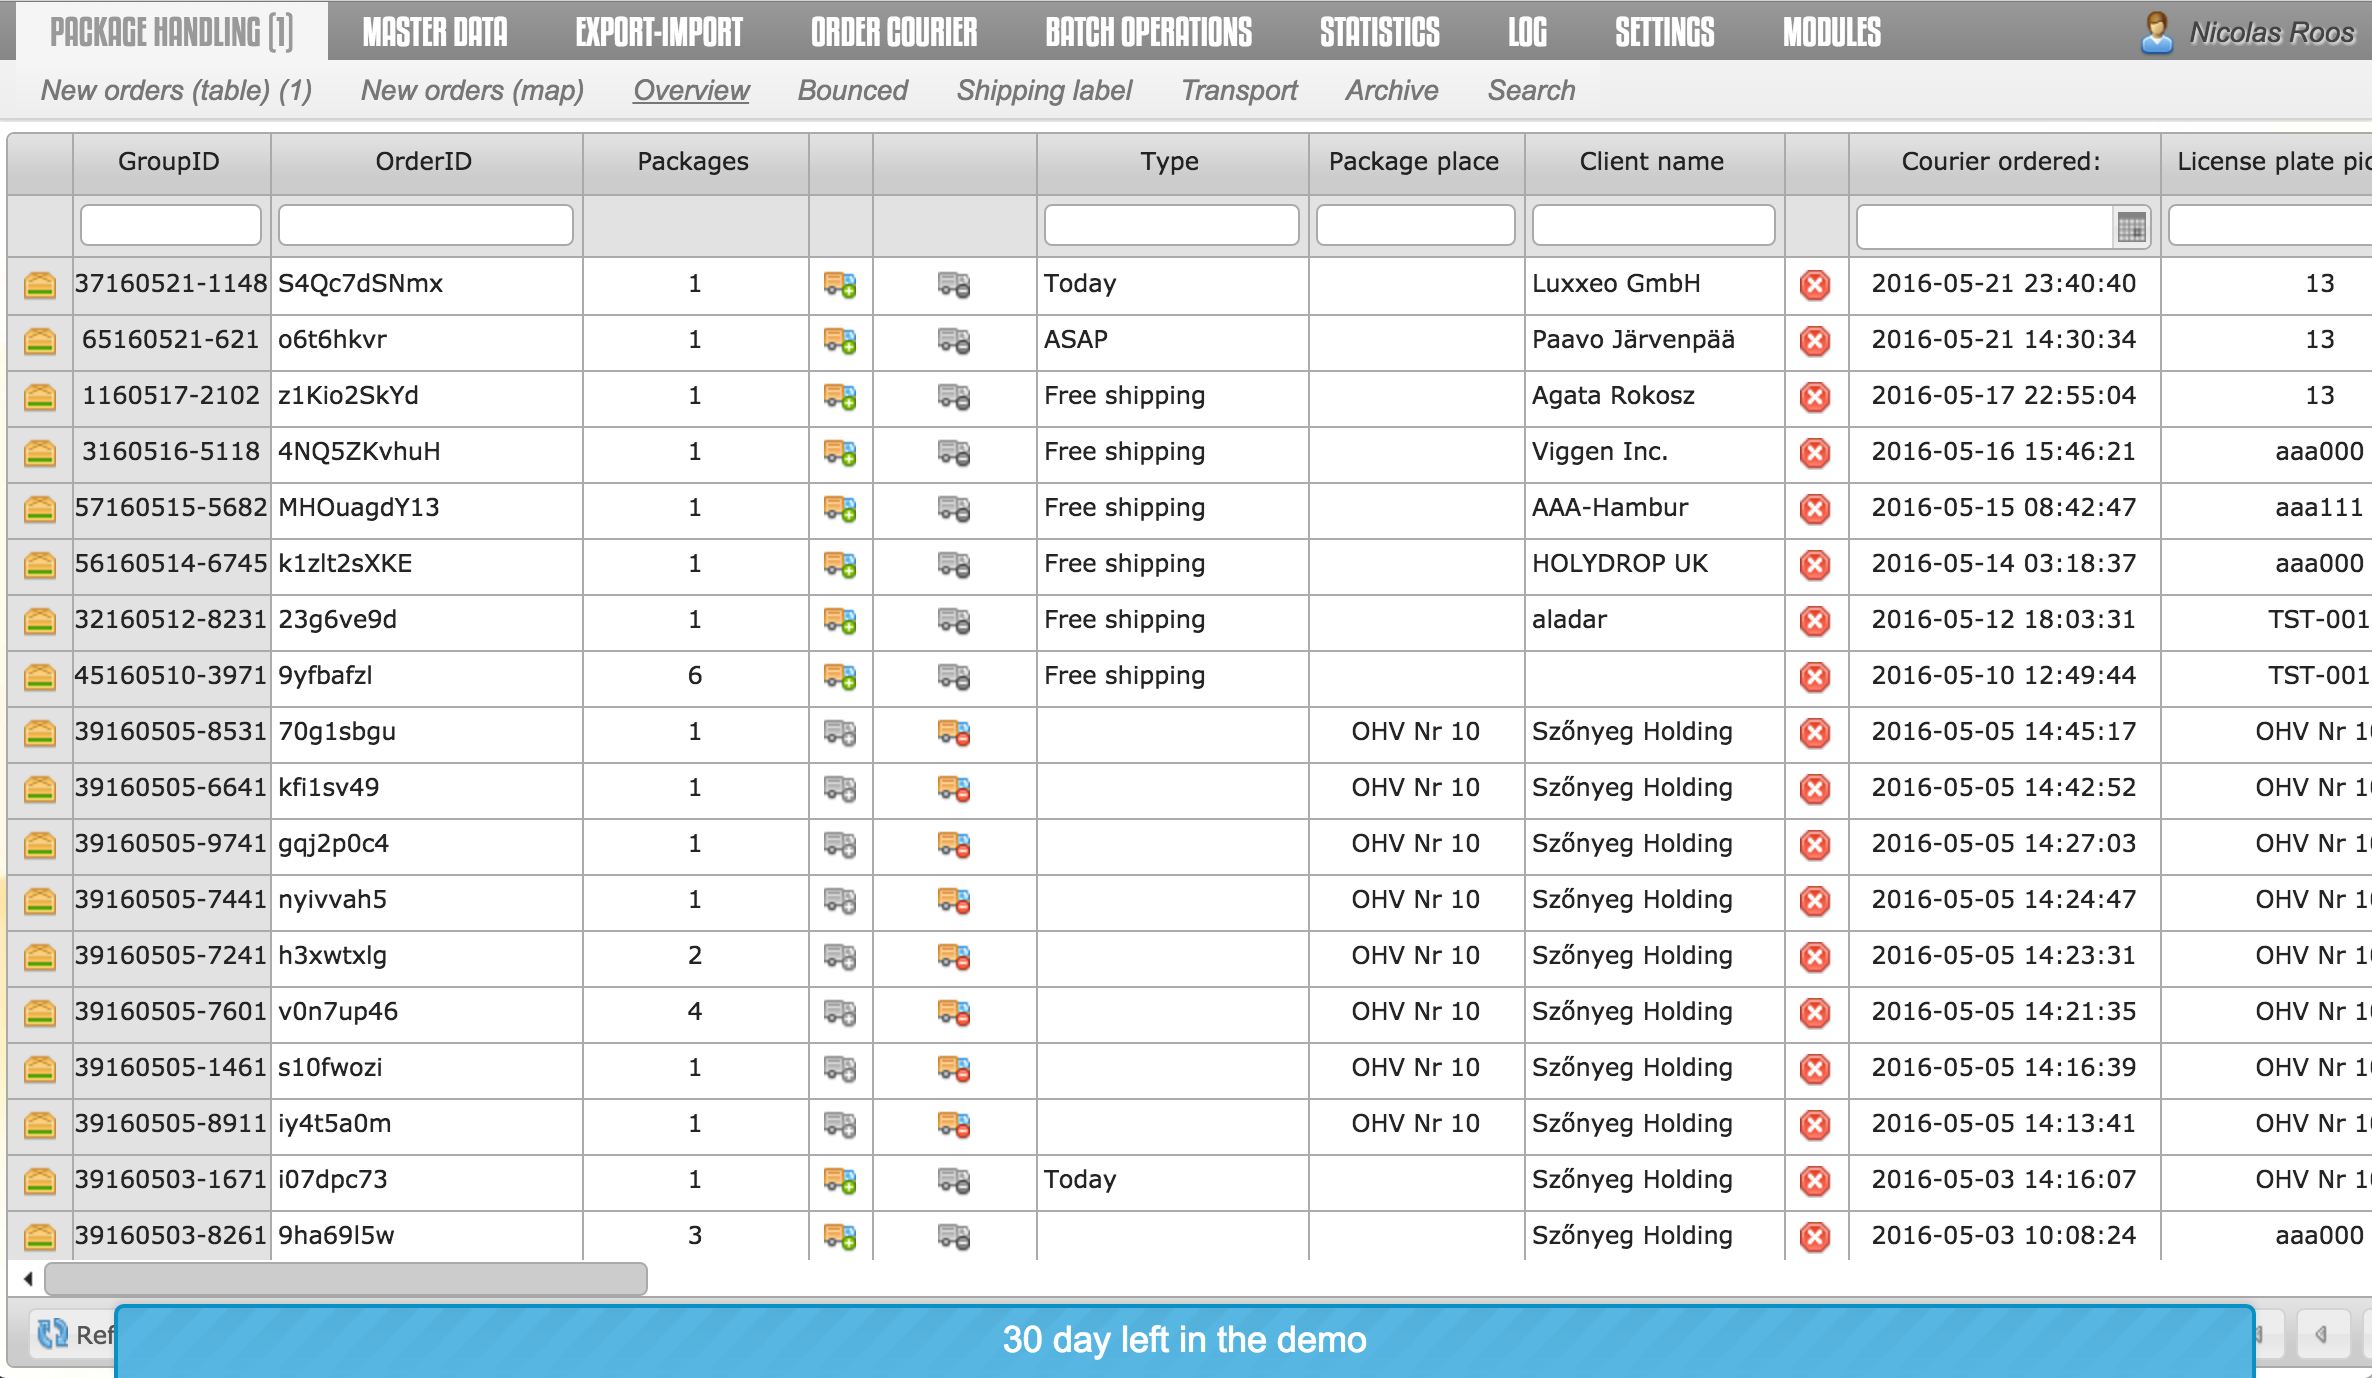
\includegraphics[width=0.66\textwidth]{images/deliveo.png}
	\caption{Auftragsmaske von Deliveo}
	\label{fig1:deliveomask}
\end{figure}

\begin{figure}[ht]
	\centering
  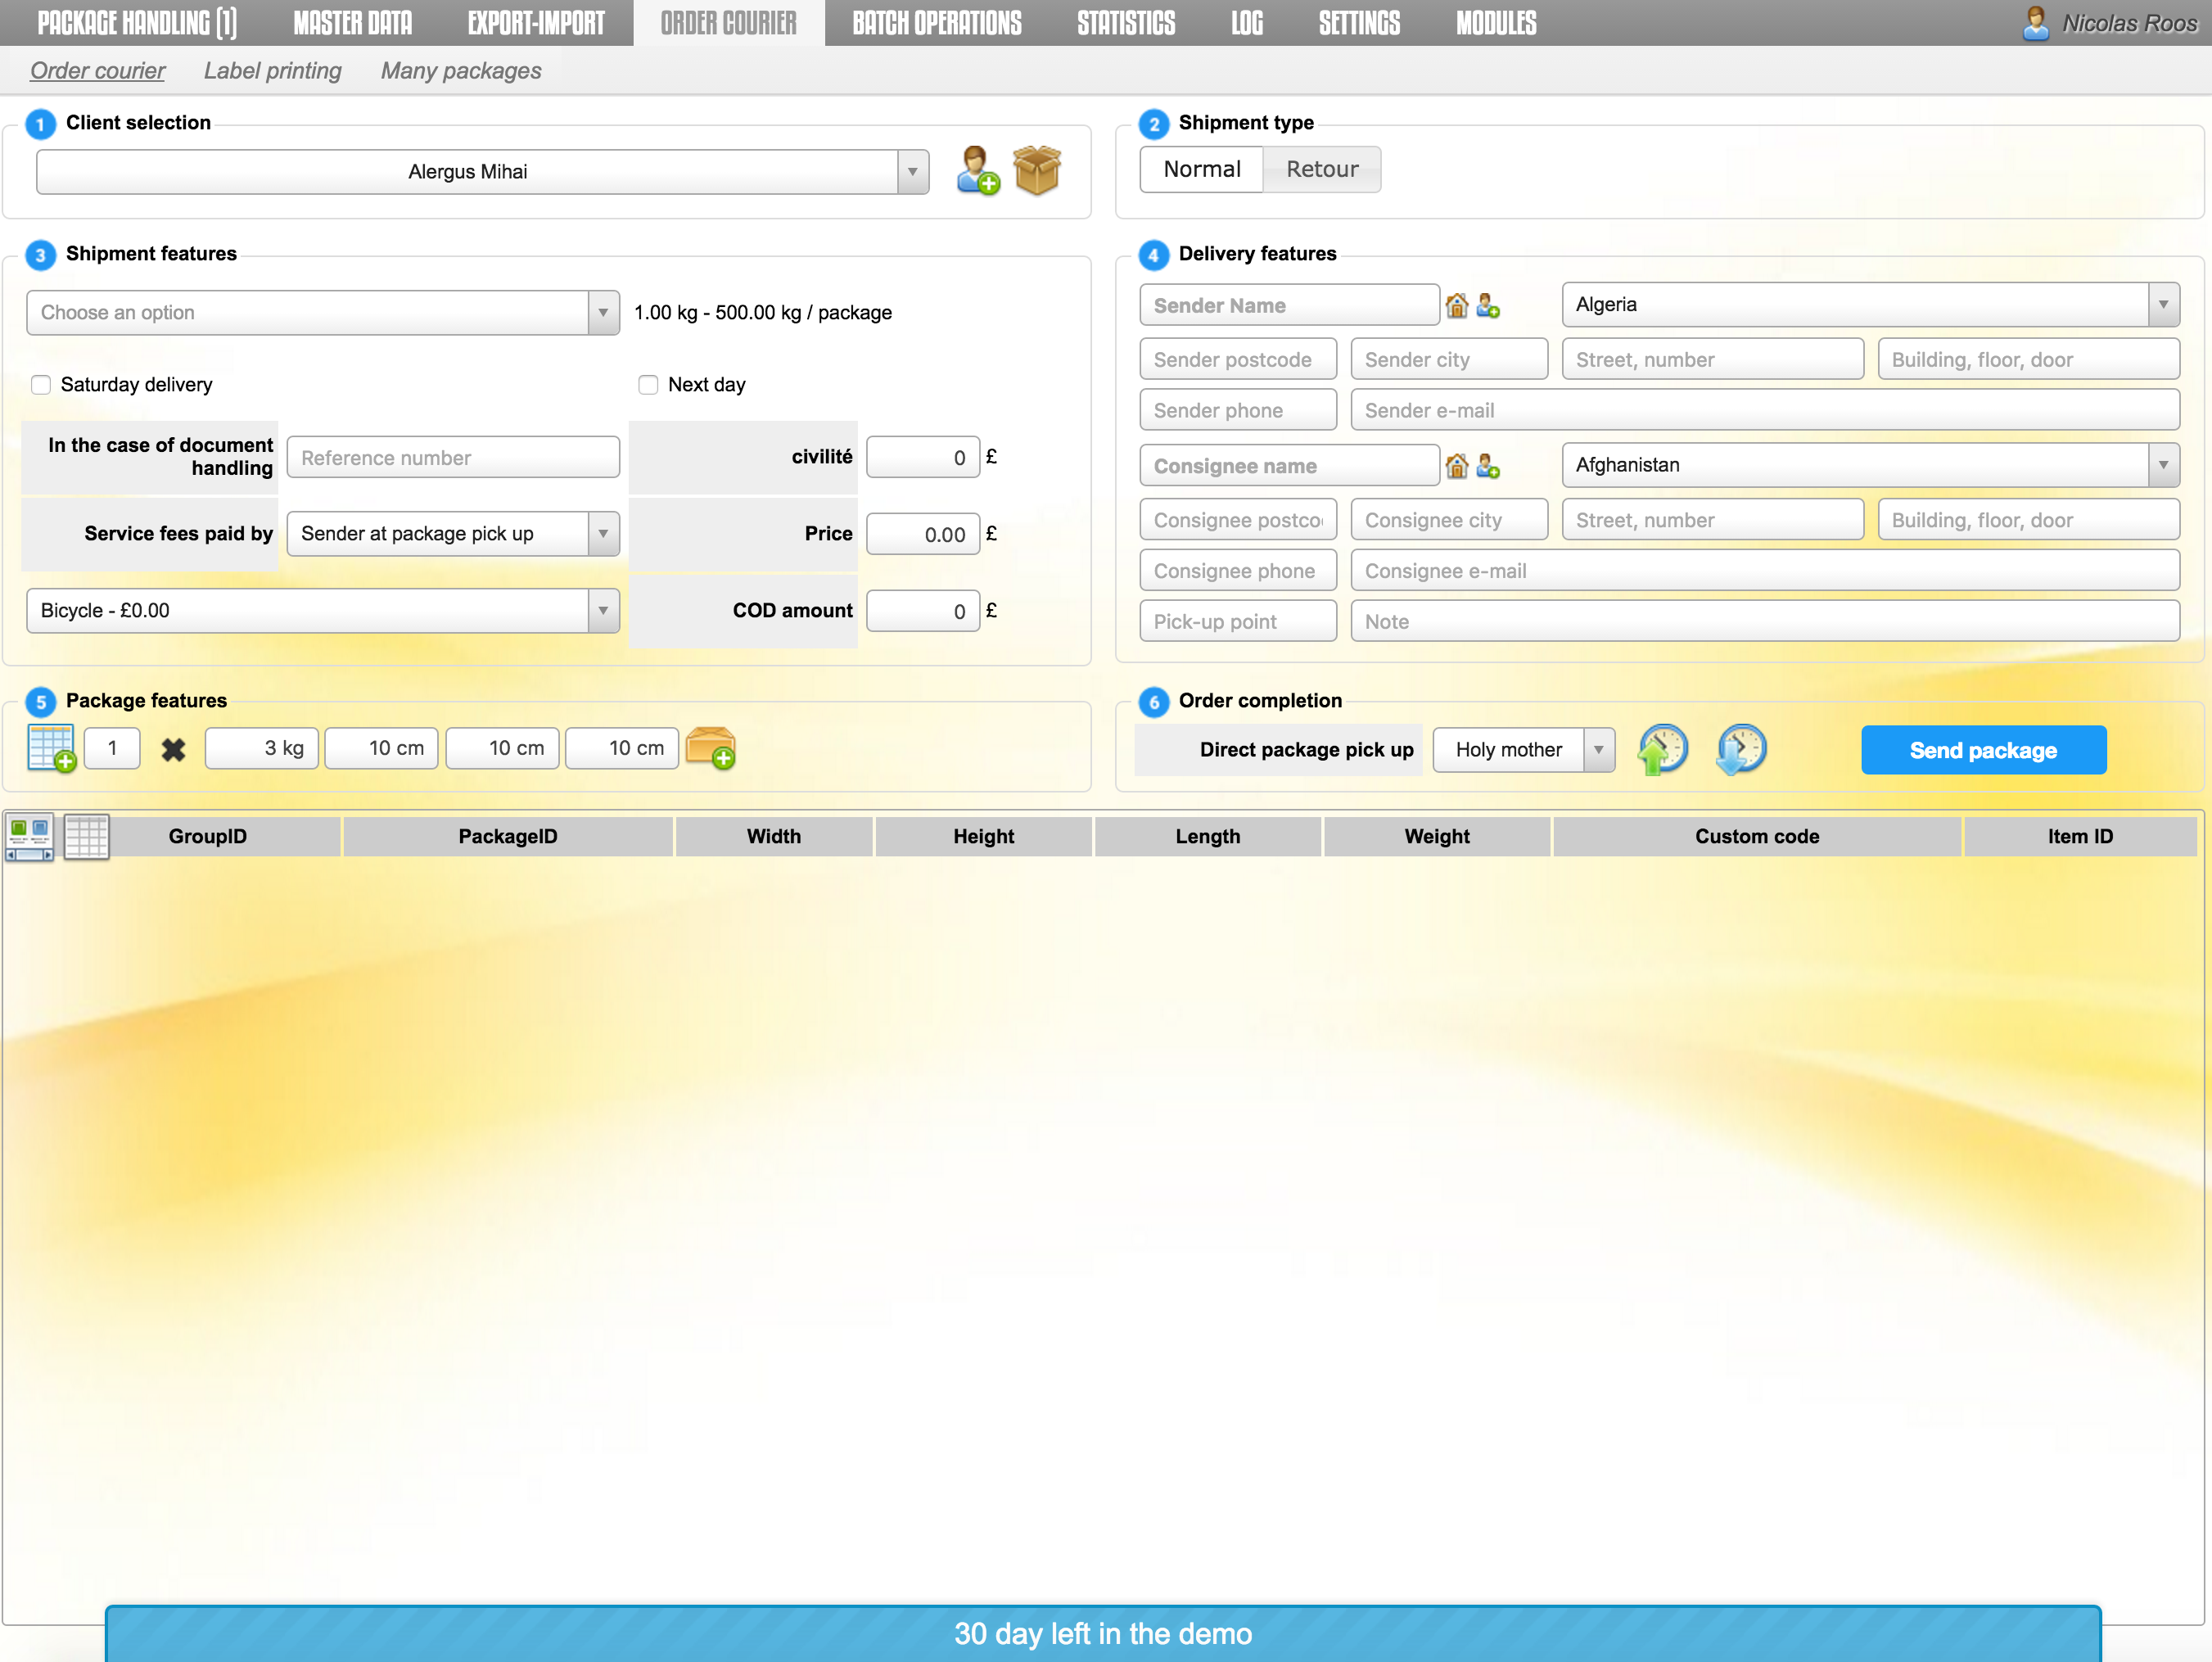
\includegraphics[width=0.66\textwidth]{images/deliveoNew.png}
	\caption{Auftragsmaske für das Erstellen eines neuen Auftrages}
	\label{fig1:deliveonew}
\end{figure}

Deliveo offeriert eine eigene API. Obwohl die Dokumentation dieser Schnittstelle in Ungarisch geschrieben ist, ist es möglich, damit einen Auftrag zu erstellen. Das System bietet eine Benutzerverwaltung an, welche aber nur eine Authentifizierung anbietet und keine Autorisierung betreibt.

\subsection{eCourier}
Die Webapplikation eCourier bietet eine Softwarelösung für KEP-Dienstleister an. Sie wurde von Bamboo-Software, einem Entwicklungsunternehmen in Berlin, hergestellt. Die Software bietet ähnliche Funktionen wie LoBo und Deliveo an. Im Folgenden eine nicht abgeschlossene Liste mit Funktionen von eCourier\footnote{ Informationen direkt von der Webseite des Herstellers. \url{https://bamboo-software.de/ecourier}}
\begin{itemize}
	\item Geeignet für Stadtkurier / Direktkurier / nationaler  und internationaler Expressversand
	\item Anbindungen an Tom Tom und AIS vorhanden
	\item Schnittstellen unter anderem zu UPS, Der Kurier, KEP AG, FedEx, Ilonexs, GEL, GLS, time:matters
\end{itemize}
Aufgrund mangelnder Testmöglichkeiten - Bamboo-Software bietet für Evaluationszwecken keine Testinstallation an - konnte eCourier im Rahmen dieser Bachelorarbeit nicht getestet werden. Die Benutzeroberfläche\footnote{Siehe Abbildung \ref{fig1:bamboonew}} jedoch sieht vielversprechend aus und die direkte Anbindung an time:matters ist äusserst interessant.

\begin{figure}[ht]
	\centering
  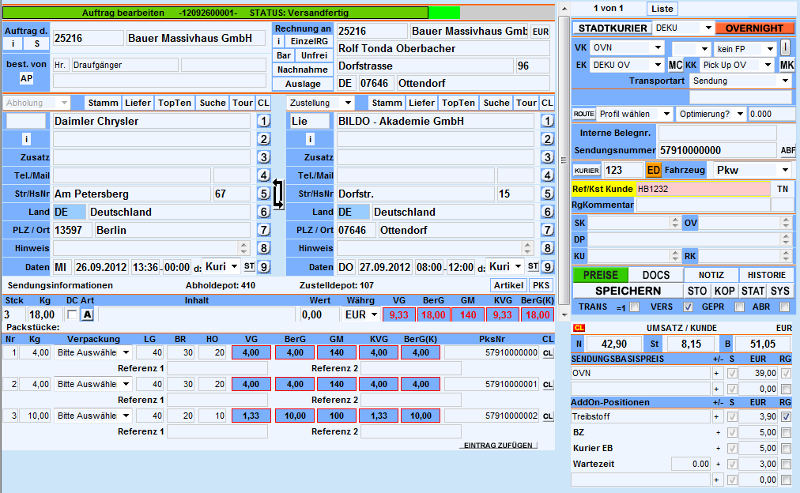
\includegraphics[width=0.66\textwidth]{images/bambooNew.jpg}
	\caption{Auftragsmaske für das Erstellen eines neuen Auftrages}
	\label{fig1:bamboonew}
\end{figure}

\subsection{Fazit}
Obschon die beiden analysierten Softwarelösungen, die aktuelle auf dem Mark zu finden sind, einen positiven Eindruck hinterlassen und die gleiche Funktionalität, welche die im Rahmen dieser Bachelorarbeit zu entwickelnde, Benutzeroberfläche benötigt, wie LoBo anbieten, sind beide Lösungen ungeeignet. Die Lösung von Bamboo-Software wurde bei der Gründung von ImagineCrago zusammen mit LoBo evaluiert und hat den Anforderungen des Start-Ups nicht genügt. Die ganze Backoffice-Funktionalität wird zwar nicht für die zu entwickelnde Benutzeroberfläche benötigt, ist aber ein grosser Bestandteil für die Wahl eines Backend. Die Benutzeroberfläche von Deliveo ist Menschen mit weniger Erfahrung zuzumuten. Aber aufgrund der fehlenden Möglichkeit Benutzer zu autorisieren, benötigt auch diese Lösung eine eigene Webapplikation, bei welcher der Benutzer nur Aufträge aufgeben kann und keine anderen Berechtigungen hat. Zusätzlich unterhält ImagineCargo enge Beziehungen zum Entwickler von LoBo und hat dadurch die Möglichkeit, zukünftige Entwicklungen zu beeinflussen. Der Entwickler von LoBo hat auch Interesse an einer \textit{White Label}\footnote{ Eine \textit{White Label} Lösung ist ohne Marke und kann vom Kunden selbst angepasst werden.} Version der im Rahmen dieser Bachelorarbeit zu entwickelnden Webapplikation bekundet. Diese Situation bietet viele Möglichkeiten für Anpassungen in LoBo, was ein bedeutend grösserer Vorteil ist als die zuvor erwähnten von Deliveo und eCourier. Dieses Fazit ist in der nicht funktionalen Anforderung NFREQ-002 festgehalten.